\chapter{Signals}

The signal system is implemented to somewhat comfort with \acs{POSIX} threads
and process signaling. This means that signals can be sent to both processes as
well as threads. Signals are passed to signal receiving entities in forwarding
fashion, a bit like how packet forwarding works.

\begin{figure}
  \center
  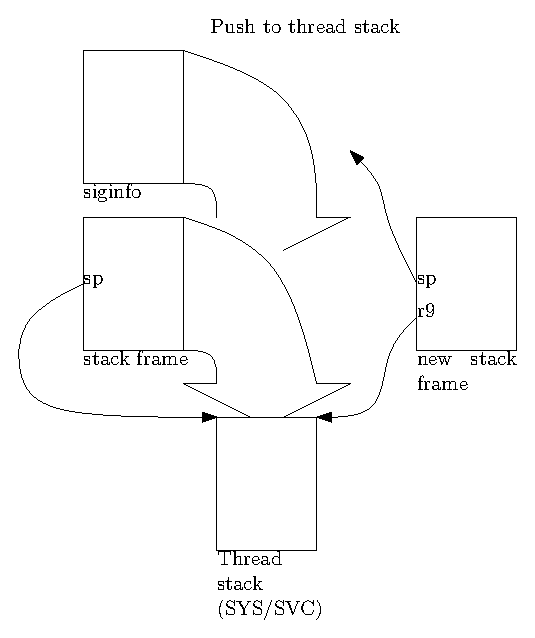
\includegraphics[width=7cm]{pics/signal_stack}
  \caption{Signal stack.}
  \label{figure:sigstack}
\end{figure}
